\chapter{Mission results}
At $3^{rd}$ of December 2018, PW-Sat2 was launched on \SI{590}{\kilo\meter} orbit on-board Falcon9 rocket from SpaceX company. 

\section{Lanuch and Early Operations Phase}
During first hours after launch, PW-Sat2 was inside the container, completery turned off by the kill-switch. 4 hours after the launch, it was deployed and turned on automatically. On-Board software, after silent period of \SI{30}{\minute} performed antenna deployment procedure and started transmitting beacon data every \SI{60}{\second}.

%TODO http://k4kdr.github.io/
Beacon data (consisting of satellite telemetry) was received first by Scott Chapman (K4KDR) from United States of America at 6:10 am the day after launch. Later, during the first couple of days of orbital operations the Bus and Payload commissionings were performed.

During first sessions, satellite was transmitting with \SI{1200}{\bps} downlink speed, providing reliable radio link. PW-Sat2 took first polish satellite photograph \ref{TODO} at \si{5^{th}} of December 2018. It was taken by a part of camera built-in tests and downloaded on request from ground.


\section{Doppler correction}
During the launch, \si{64} satellites were launched together and were separated from the upper stage of the rocket by spring actions. At first, they were flying together and with the time, they were further apart from each other. Figure \ref{TODO} show the on-orbit position of the satellites on \si{25^{th}} day after the launch. Doppler effect estimation was performed during every pass, with increased accuracy. Typical method for selecting an satellite object from a set of different ones is done by applying Doppler correction to the received signal spectrum, for every object in the field of view, and later choosing the most suited one. 

Signal before and after Doppler correction is shown in the figure \ref{Doppler_correction_gqrx}.

\begin{figure}
    \centering
    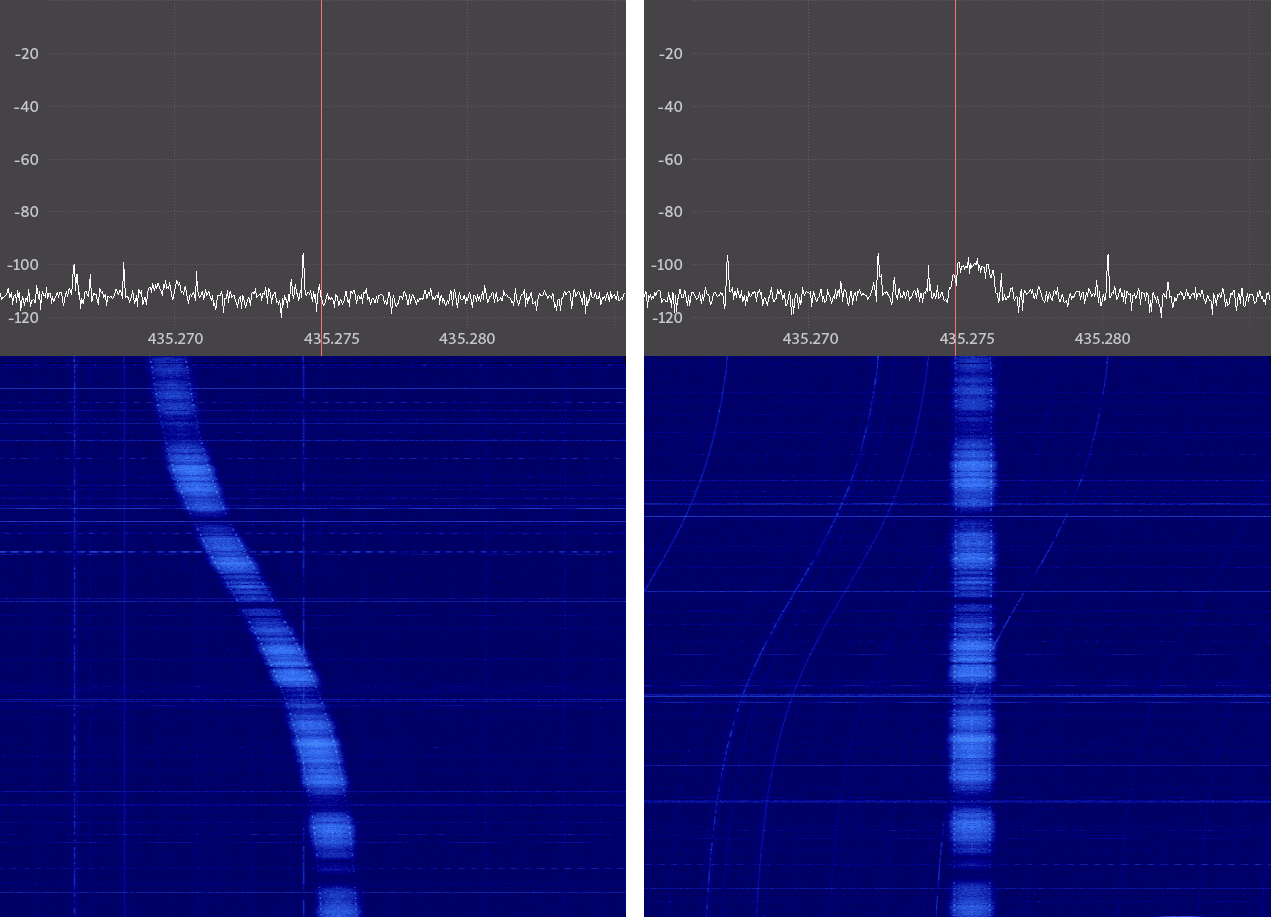
\includegraphics[width=0.65\paperwidth]{img/6/doppler_correction.png}
    \caption{Doppler correction.}
    \label{Doppler_correction_gqrx}
\end{figure}

\section{Link budget estimation}


\section{Main mission results}


